\documentclass[a4paper,12pt]{article}

\usepackage[T1]{fontenc}
\usepackage[utf8]{inputenc}
\usepackage{graphicx}
\usepackage{xcolor}
\renewcommand\familydefault{\sfdefault}
\usepackage{tgheros}
\usepackage[defaultmono]{droidmono}
\usepackage{amsmath,amssymb,amsthm,textcomp}
\usepackage{enumerate}
\usepackage{multicol}
\usepackage{tikz}
\usepackage{float}
\usepackage{geometry}
\usepackage{dirtytalk}
\geometry{left=25mm,right=25mm,%
bindingoffset=0mm, top=20mm,bottom=20mm}
\linespread{1.3}
\newcommand{\linia}{\rule{\linewidth}{0.5pt}}

% custom theorems if needed
\newtheoremstyle{mytheor}
    {1ex}{1ex}{\normalfont}{0pt}{\scshape}{.}{1ex}
    {{\thmname{#1 }}{\thmnumber{#2}}{\thmnote{ (#3)}}}

\theoremstyle{mytheor}
\newtheorem{defi}{Definition}

% my own titles
\makeatletter
\renewcommand{\maketitle}{
\begin{center}
\vspace{2ex}
{\huge \textsc{\@title}}
\vspace{1ex}
\\
\linia\\
\@author \hfill \@date
\vspace{4ex}
\end{center}
}
\makeatother
%%%

% custom footers and headers
\usepackage{fancyhdr}
\usepackage{hyperref}
\usepackage{listings}
\pagestyle{fancy}
\lhead{}
\chead{}
\rhead{}
\lfoot{Sztuczna Inteligencja, Sprawozdanie nr 9}
\cfoot{}
\rfoot{Strona \thepage}
\renewcommand{\headrulewidth}{0pt}
\renewcommand{\footrulewidth}{0pt}
\usepackage[tablename=Tablica]{caption}
%

%%%----------%%%----------%%%----------%%%----------%%%

\begin{document}

\title{SI - SPRAWOZDANIE LAB nr 9}

\author{Maciej Budzowski, dzienne, grupa L5}

\date{01/06/2020}

\maketitle
Link do pliku .tex na platformie OverLeaf: \textcolor{red}{\href{https://www.overleaf.com/read/gtjhbdddtygc}{OVERLEAF}}

\section*{Analiza danych przy użyciu sieci Kohonena}

\section*{Użyty zbiór danych}
\linia\\

Analiza została wykonana na zbiorze \textbf{\emph{Wholesale customers}}, linki do źródeł zamieszczam poniżej:\\
\textcolor{red}{\href{https://archive.ics.uci.edu/ml/machine-learning-databases/00292/Wholesale\%20customers\%20data.csv}{DANE (PLIK)}} (link prowadzi do oryginalnego pliku)\\
\textcolor{red}{\href{https://archive.ics.uci.edu/ml/datasets/Wholesale+customers}{DANE (STRONA)}} (link prowadzi do strony datasetu)\\

\textbf{Opis/temat zbioru:} Wedle strony datasetu: \say{Zestaw danych odnosi się do klientów dystrybutora hurtowego. Obejmuje roczne wydatki w jednostkach monetarnych (m.u.) na różne kategorie produktów}\\

\textbf{Autor:}\\
Margarida G. M. S. Cardoso, margarida.cardoso '@' iscte.pt, ISCTE-IUL, Lisbon, Portugal\\

\textbf{Parametry użytego zbioru:}\\
 - liczba obserwacji - 440\\
 - liczba cech, atrybutów - 8\\

\textbf{Lista cech w zbiorze (wedle strony):}
\begin{itemize}
  \item1) FRESH: roczne wydatki (m.u.) na świeże produkty (Liczbowe);
  \item2) MILK: roczne wydatki (m.u.) na mleczne produkty (Liczbowe);
  \item3) GROCERY: roczne wydatki (m.u.) na spożywcze produkty (Liczbowe);
  \item4) FROZEN: roczne wydatki (m.u.) na mrożone produkty (Liczbowe)
  \item5) DETERGENTS-PAPER: roczne wydatki (m.u.) na detergenty i papierowe produkty (Liczbowe)
  \item6) DELICATESSEN: roczne wydatki (m.u.) na delikatesy (Liczbowe);
  \item7) CHANNEL: klienci (kanał sprzedaży) - Horeca (Hotel/Restaurant/Cafe) lub handel detaliczny (Nominalne)
  \item8) REGION: Region - Lisbon, Oporto or Other (Nominalne) 
\end{itemize}

\section*{Przygotowanie danych}
\linia\\
 W ramach przygotowania danych do pracy nie musiałem dokonywać zmian bezpośrednio w oryginalnym pliku. Natomiast zgodnie z metodą z odbytych ćwiczeń analiza została dokonana bez nazw klas.
 
\section*{Kod}
\linia\\
\textbf{Link do projektu ze skryptem:} \textcolor{red}{\href{https://github.com/bvdzynski/up_ai-lab/tree/master/lab9_project_wholesale_customers}{GITHUB}}\\

Sieci Kohonena tworzyłem przy użyciu skryptu języka R. Opiera się on na kodzie z odbytych ćwiczeń.\\

\textbf{Proces analizy przebiega następująco (w kolejności):}
\begin{itemize}
 \item Wczytujemy plik z danymi.
 \item Pozbywamy się niepotrzebnych kolumn z nazwami klas (region i channel).
 \item Dane przekształcamy do macierzy.
 \item Definiujemy siatkę SOM.
 \item Uruchamiamy algorytm trenowania SOM
 \item Rysujemy wykresy i dokonujemy obserwacji
 \item Pozostawiamy komentarz
\end{itemize}

Obliczenia wykonywały się szybko, więc w tym przypadku nie było potrzeby automatyzacji procesu.\\

Proces wykonałem (tak jak na ćwiczeniach) w kilku próbach, przy użyciu różnych wielkości siatki SOM. Ostatecznie do próby wyciągnięcia informacji z danych zdecydowałem się (ze względu na ilość danych i otrzymywane wykresy) na siatkę 4x4.

\section*{Wyniki}
\linia\\
Poniżej przedstawiam pojedyncze wykresy dla otrzymanych danych.

\begin{figure}[H]
    \centering
    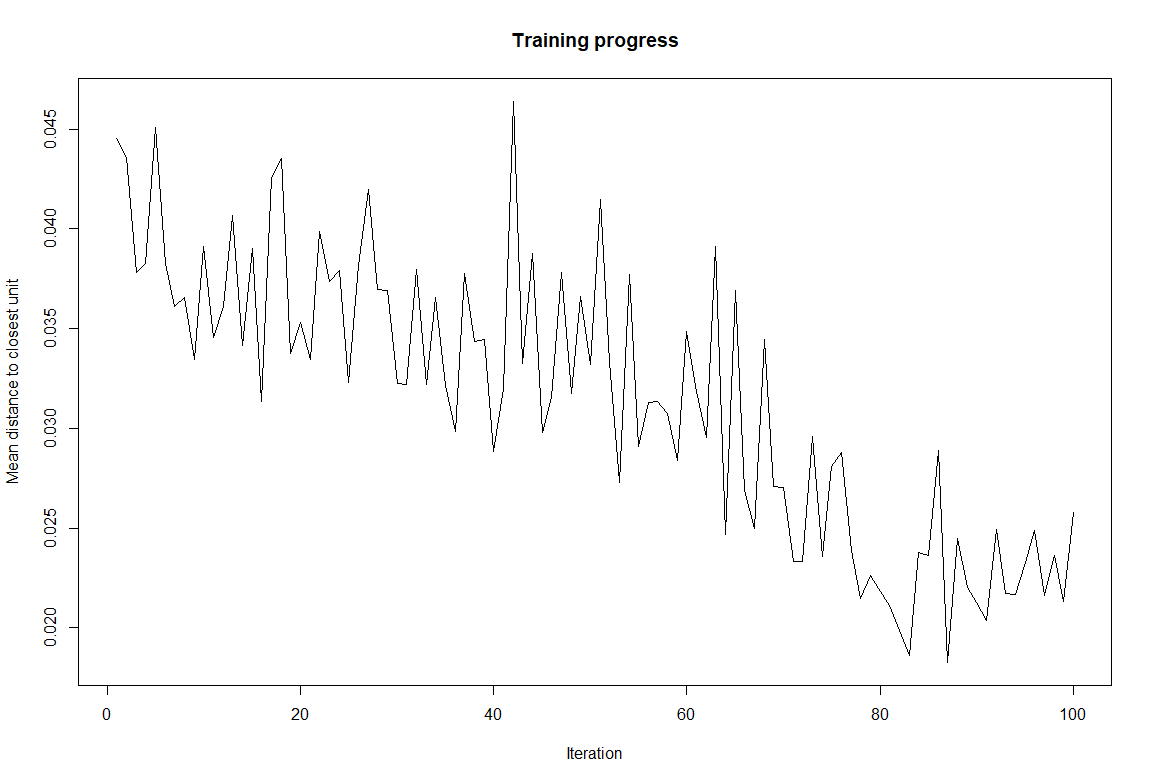
\includegraphics[width=0.75\textwidth]{lab9_sprawozdanie/plots/original/plot_changes.png}
    \caption{wykres typu: \emph{changes}}
    \label{fig:plot1}
\end{figure}
Wykres typu \emph{changes} przedstawia średnią odleglość między neuronami.\\

\begin{figure}[H]
    \centering
    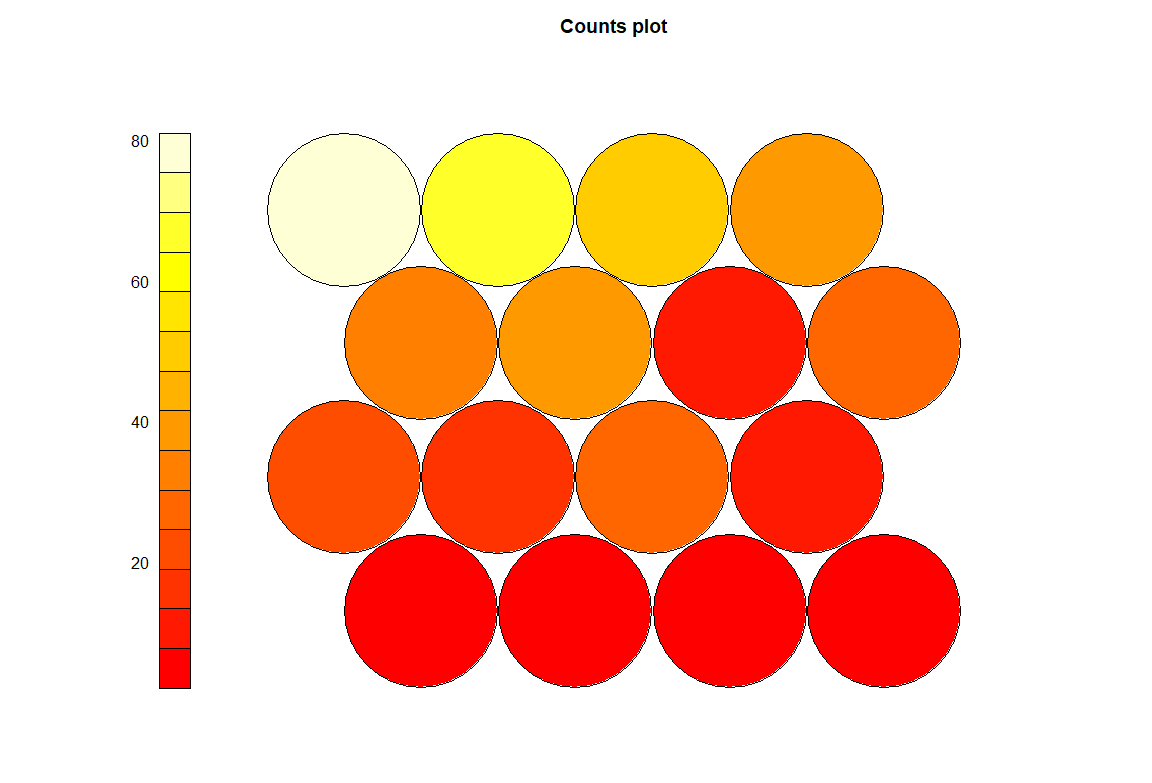
\includegraphics[width=0.75\textwidth]{lab9_sprawozdanie/plots/original/plot_count.png}
    \caption{wykres typu: \emph{count}}
    \label{fig:plot2}
\end{figure}
Wykres typu \emph{count} - każde kółko to jeden neuron, rysunek interpretuje liczbę neuronów, które są blisko danego obiektu.\\

\begin{figure}[H]
    \centering
    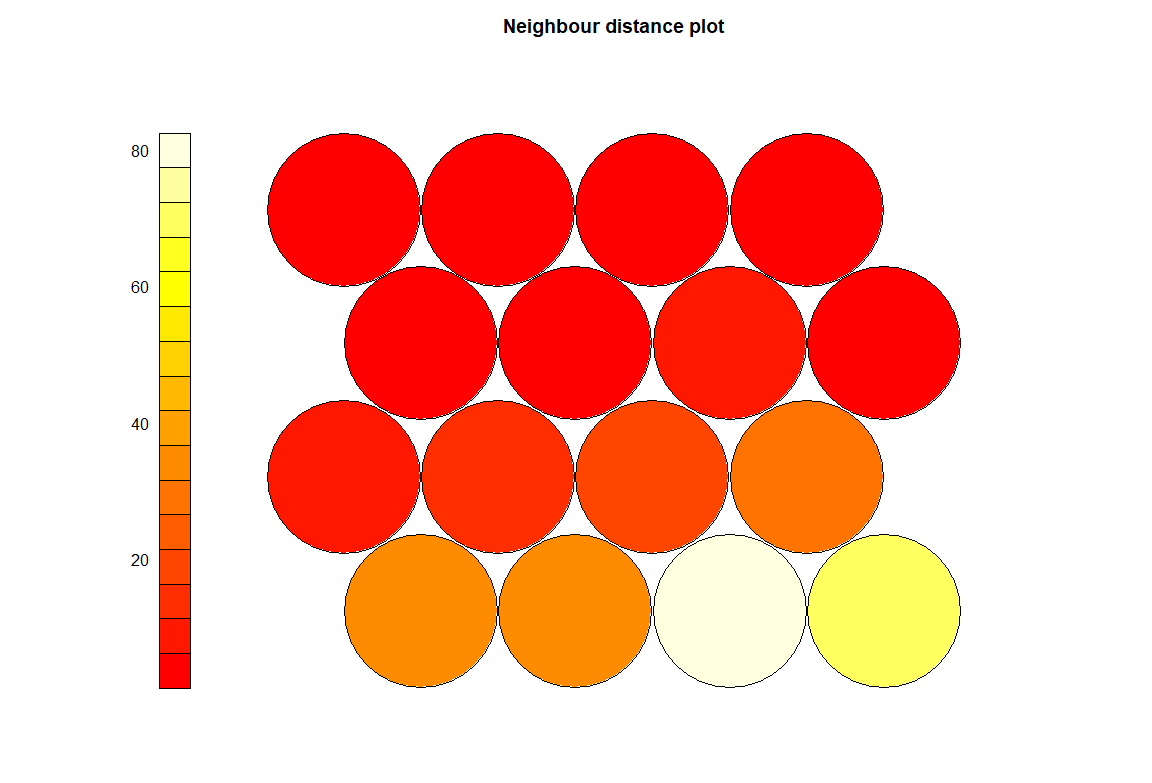
\includegraphics[width=0.75\textwidth]{lab9_sprawozdanie/plots/original/plot_dist-neighbours.png}
    \caption{wykres typu: \emph{dist.neighbours}}
    \label{fig:plot3}
\end{figure}
Wykres typu \emph{dist.neighbours} - interpretuje odległość do najbliższych sąsiadów. (obiektów)\\

\begin{figure}[H]
    \centering
    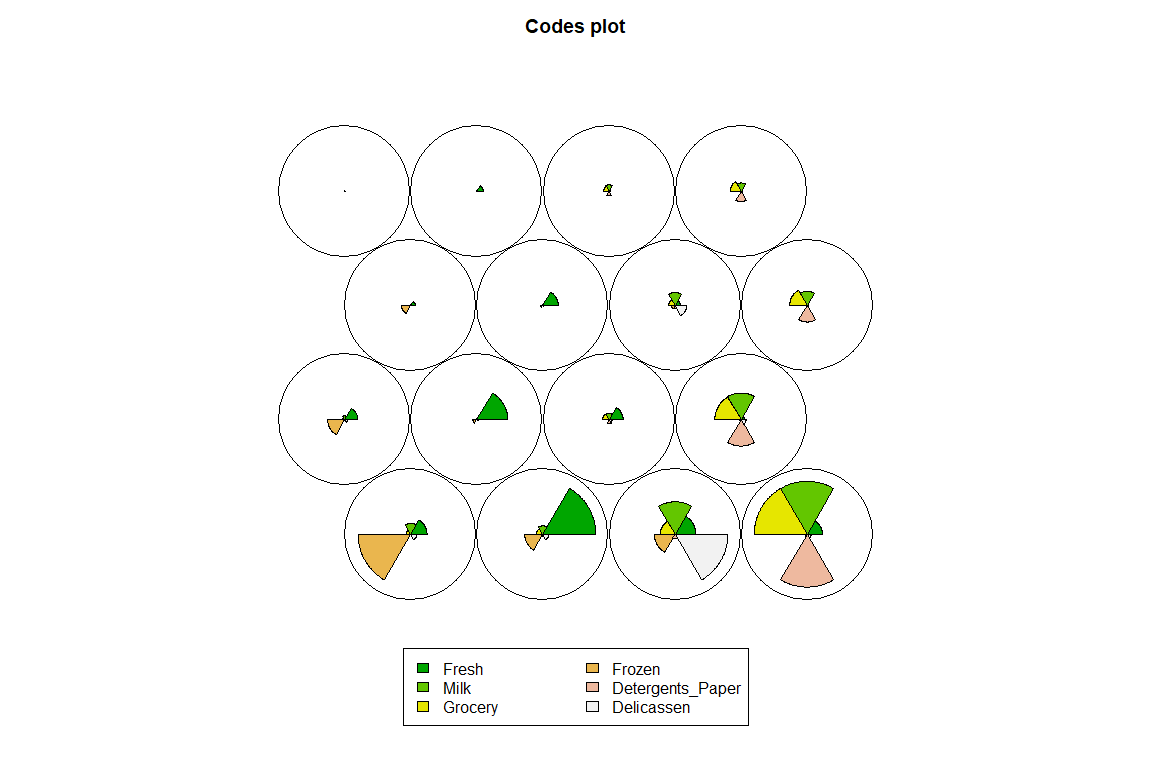
\includegraphics[width=0.75\textwidth]{lab9_sprawozdanie/plots/original/plot_codes.png}
    \caption{wykres typu: \emph{codes}}
    \label{fig:plot4}
\end{figure}
Wykres typu \emph{codes} - interpretuje udziały procentowe wartości parametrów.\\

\begin{figure}[H]
    \centering
    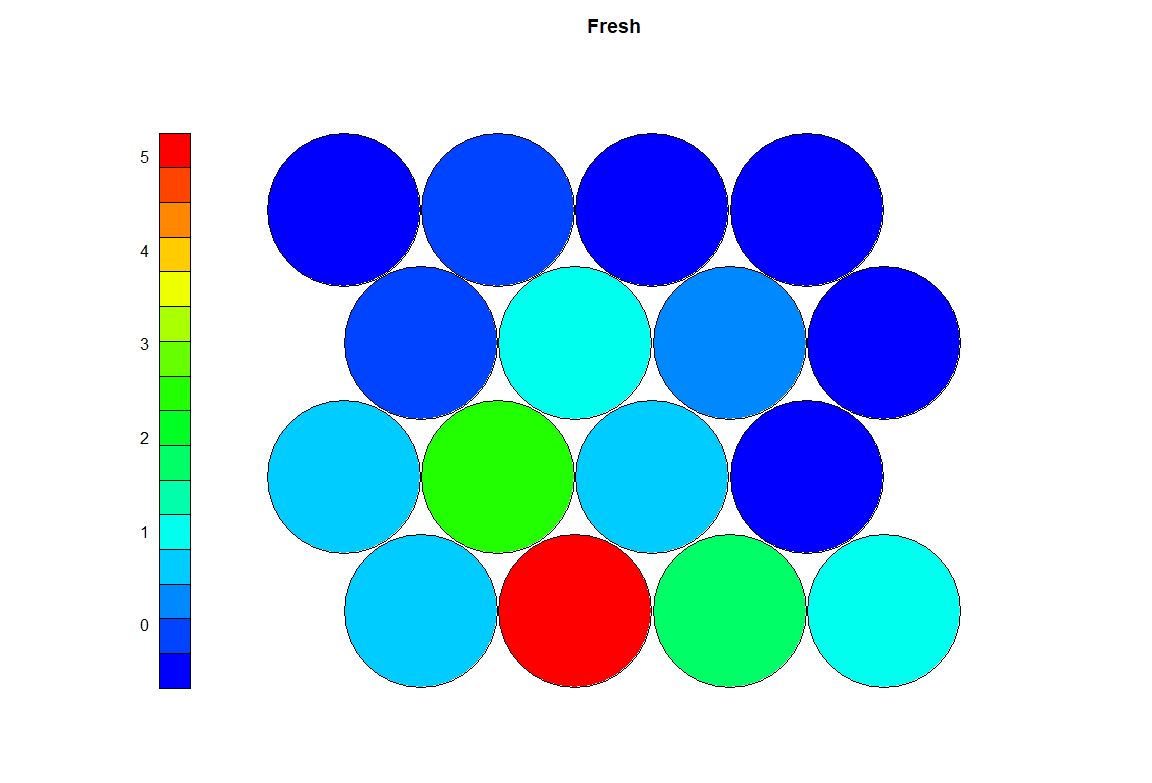
\includegraphics[width=0.75\textwidth]{lab9_sprawozdanie/plots/original/plot_var_1_fresh.png}
    \caption{wykres dla parametru \emph{Fresh}}
    \label{fig:plot5}
\end{figure}

\begin{figure}[H]
    \centering
    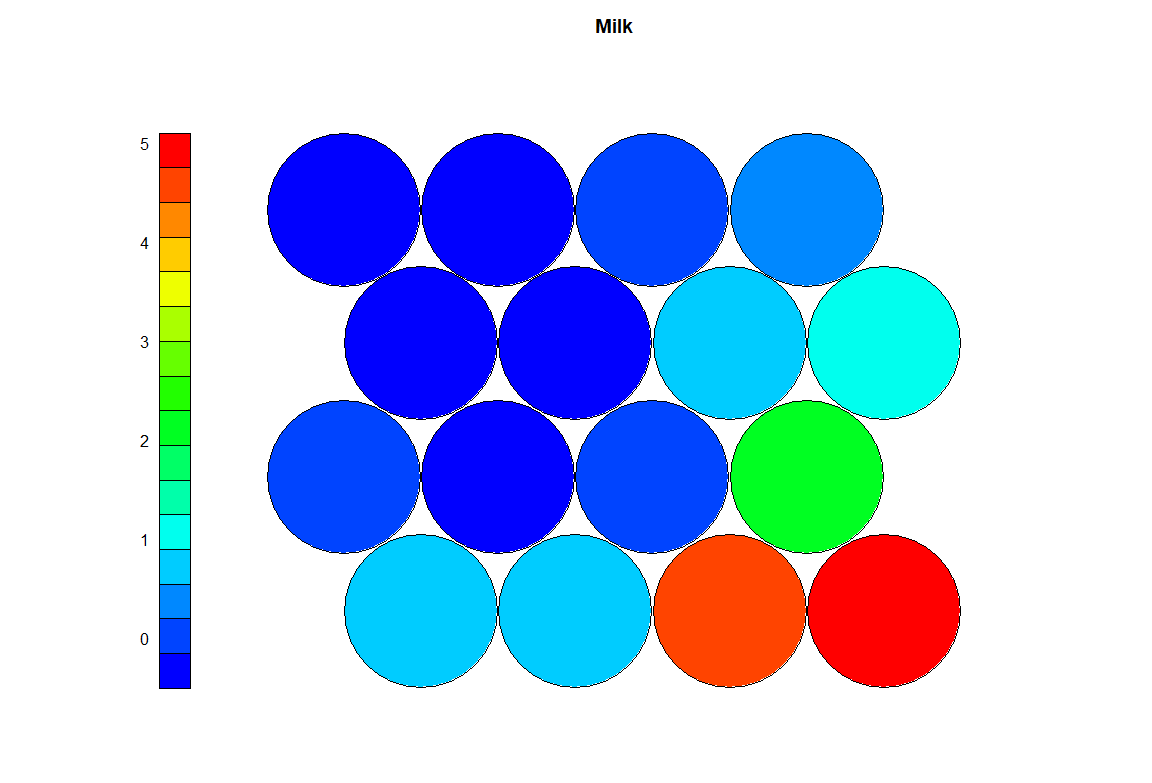
\includegraphics[width=0.75\textwidth]{lab9_sprawozdanie/plots/original/plot_var_2_milk.png}
    \caption{wykres dla parametru \emph{Milk}}
    \label{fig:plot6}
\end{figure}

\begin{figure}[H]
    \centering
    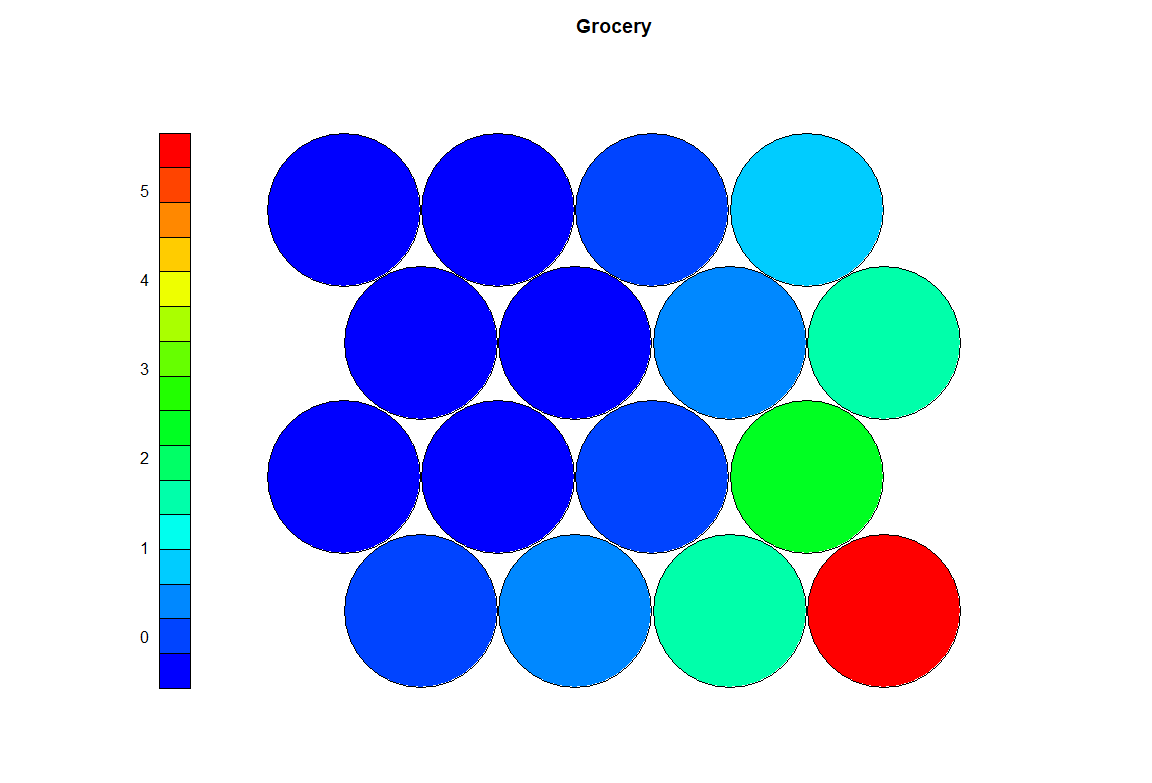
\includegraphics[width=0.75\textwidth]{lab9_sprawozdanie/plots/original/plot_var_3_grocery.png}
    \caption{wykres dla parametru \emph{Grocery}}
    \label{fig:plot7}
\end{figure}

\begin{figure}[H]
    \centering
    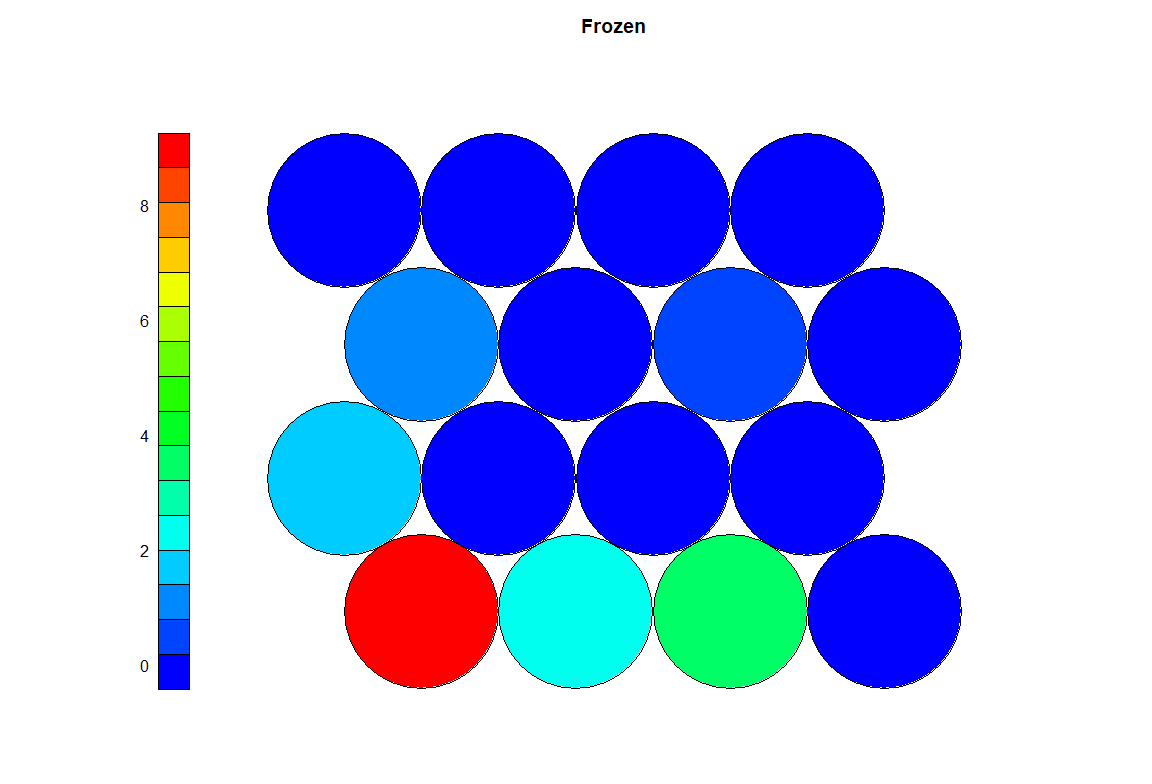
\includegraphics[width=0.75\textwidth]{lab9_sprawozdanie/plots/original/plot_var_4_frozen.png}
    \caption{wykres dla parametru \emph{Frozen}}
    \label{fig:plot8}
\end{figure}

\begin{figure}[H]
    \centering
    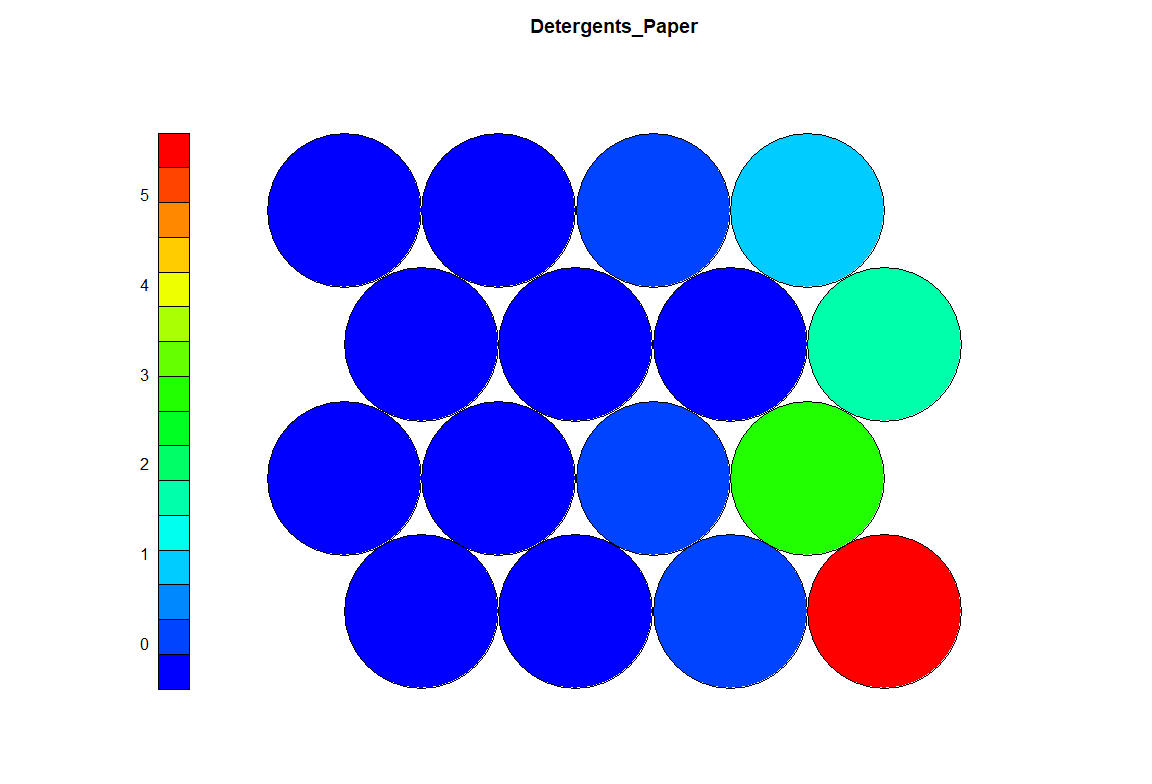
\includegraphics[width=0.75\textwidth]{lab9_sprawozdanie/plots/original/plot_var_5_detergents.png}
    \caption{wykres dla parametru \emph{Detergents and Paper}}
    \label{fig:plot9}
\end{figure}

\begin{figure}[H]
    \centering
    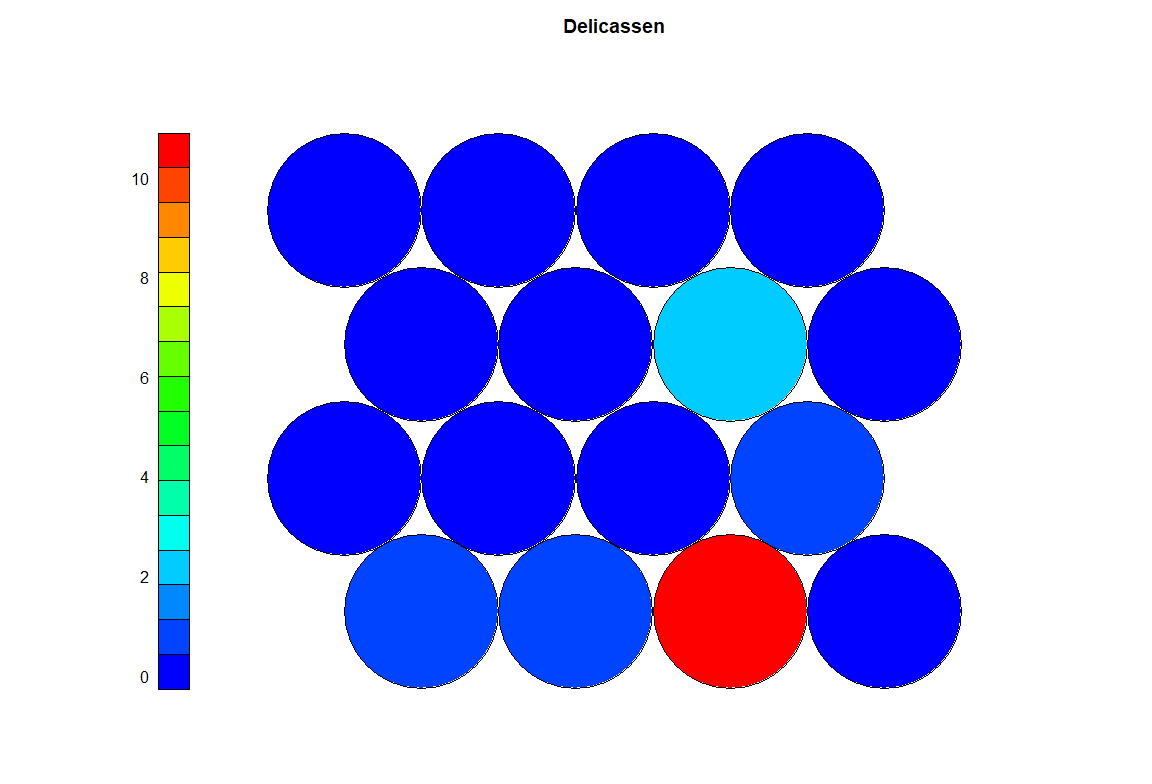
\includegraphics[width=0.75\textwidth]{lab9_sprawozdanie/plots/original/plot_var_6_delicassen.png}
    \caption{wykres dla parametru \emph{Delicassen}}
    \label{fig:plot10}
\end{figure}

\begin{figure}[H]
    \centering
    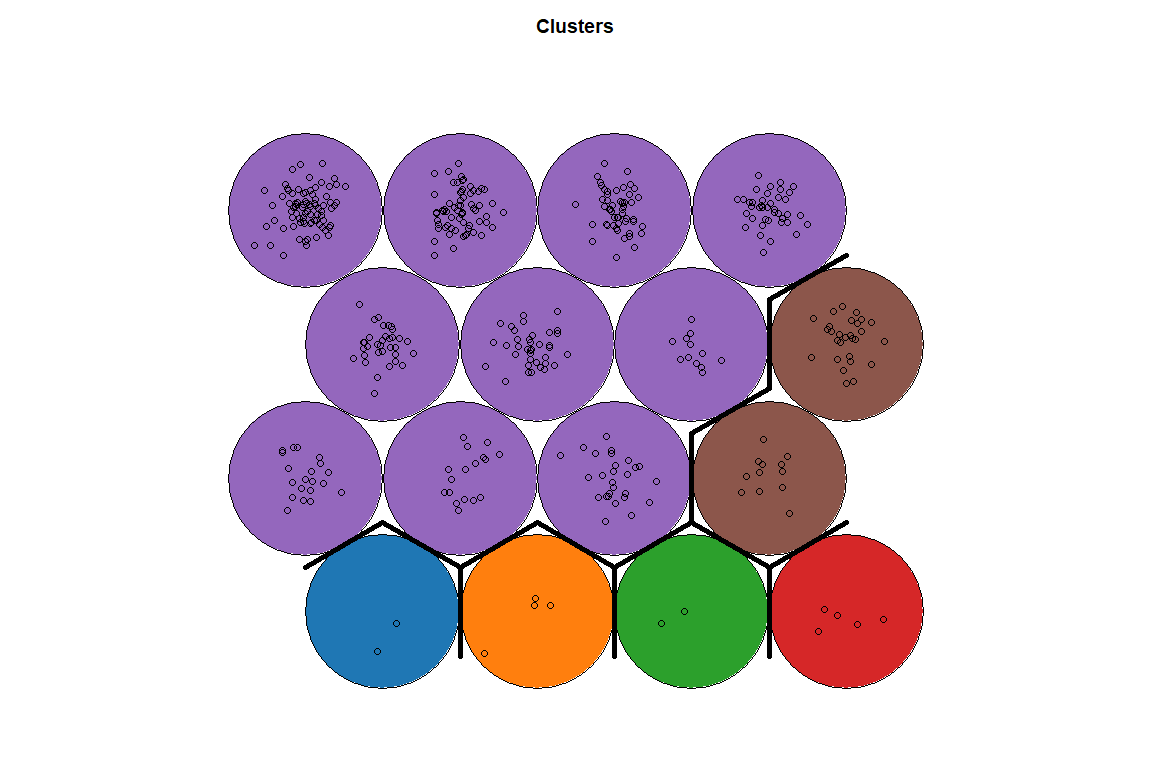
\includegraphics[width=0.75\textwidth]{lab9_sprawozdanie/plots/original/plot_clusters.png}
    \caption{grupy, które zostały uzyskane metodą klasteryzacji hierarhicznej}
    \label{fig:plot11}
\end{figure}

\section*{Wnioski, obserwacje}

Wykresy nałożyłem na siebie przy użyciu programu GIMP odpowiednio dopasowując wartość parametru "krycie".

Porównując ze sobą wykresy w poszukiwaniu korelacji znalazłem 2 możliwości, które są - moim zdaniem - warte zanotowania. Moim zdaniem, że najbardziej przydatnym wykresem, jest wykres typu \emph{codes}.

\begin{figure}[H]
    \centering
    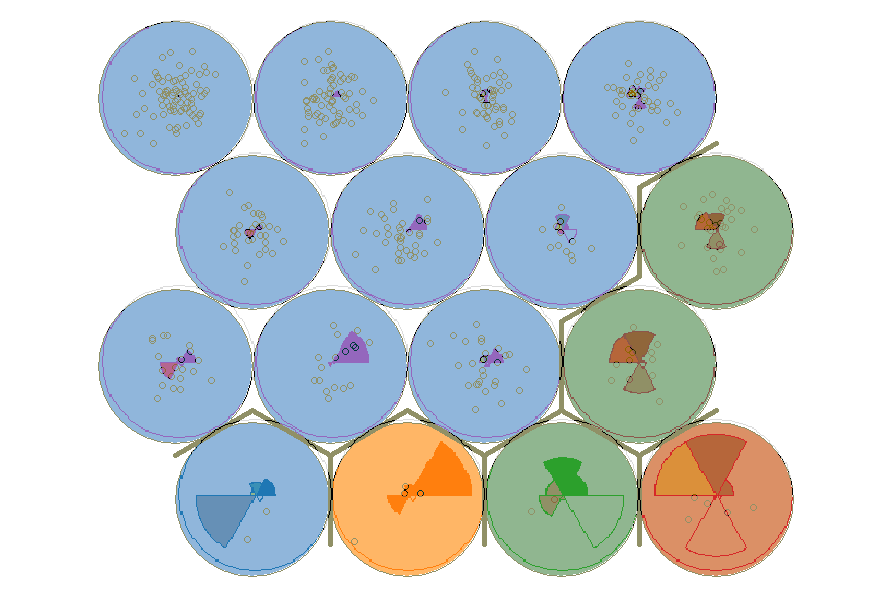
\includegraphics[width=0.75\textwidth]{lab9_sprawozdanie/plots/mixed/plots_cluster+codes.png}
    \caption{zmiksowane wykresy \emph{cluster} i \emph{codes}}
    \label{fig:plot12}
\end{figure}

W przypadku rysunku 12 mamy zmiksowane wykresy \emph{cluster} i \emph{codes}. Jako, że dane dotyczą wydatków na różne rodzaje produktów przez klientów na określonym obszarze, możemy dojść do następujących wniosków:
\begin{itemize}
 \item Mały odsetek obiektów stanowi znaczną część wydatków.
 \item W grupach, które zostały utworzone metodą klasteryzacji hierarchicznej można zauważyć tendencję do kupowania określonego rodzaju produktu w dużej ilości (czerwona - grocery/detergents, zielona - milk/delicassen, pomarańczowa - fresh).
 \item Grupa niebieska stanowi większość obiektów, natomiast stanowi ona stosunkowo mały procent w całości wydatków. Można przewidywać, że mamy tutaj do czynienia z małymi biznesami.
 \item Grupa czerwona jest "elitą" - jest to kilka obiektów, które stanowią duży procent w całości wydatków. Można przewidywać, że są to duże przesiębiorstwa.
\end{itemize}

\begin{figure}[H]
    \centering
    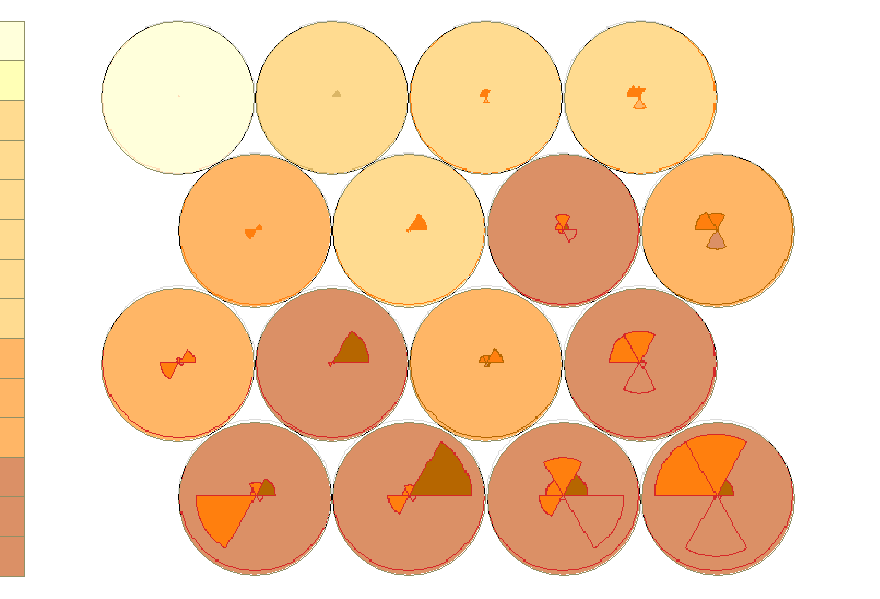
\includegraphics[width=0.75\textwidth]{lab9_sprawozdanie/plots/mixed/plots_codes+count.png}
    \caption{zmiksowane wykresy \emph{codes} i \emph{count}}
    \label{fig:plot13}
\end{figure}

W przypadku rysunku 13 mamy zmiksowane wykresy \emph{codes} i \emph{count}. Znajdujemy tutaj dodatkowe potwierdzenie poprzednich obserwacji. Stosunkowo mała ilość obiektów stanowi wysoki procent w całości wydatków. Natomiast obiekty stanowiące większość (od środka do lewego górnego rogu) stanowi mały procent w całości wydatków.

\end{document}